\newpage
\section{Theoretical Analysis}
\label{sec:analysis}

ection, the circuit is analyzed theoretically, according to the ideal op-amp model (Z i = ∞
and Z o = 0), resulting in the following equation
\begin{figure}[ht!] \centering
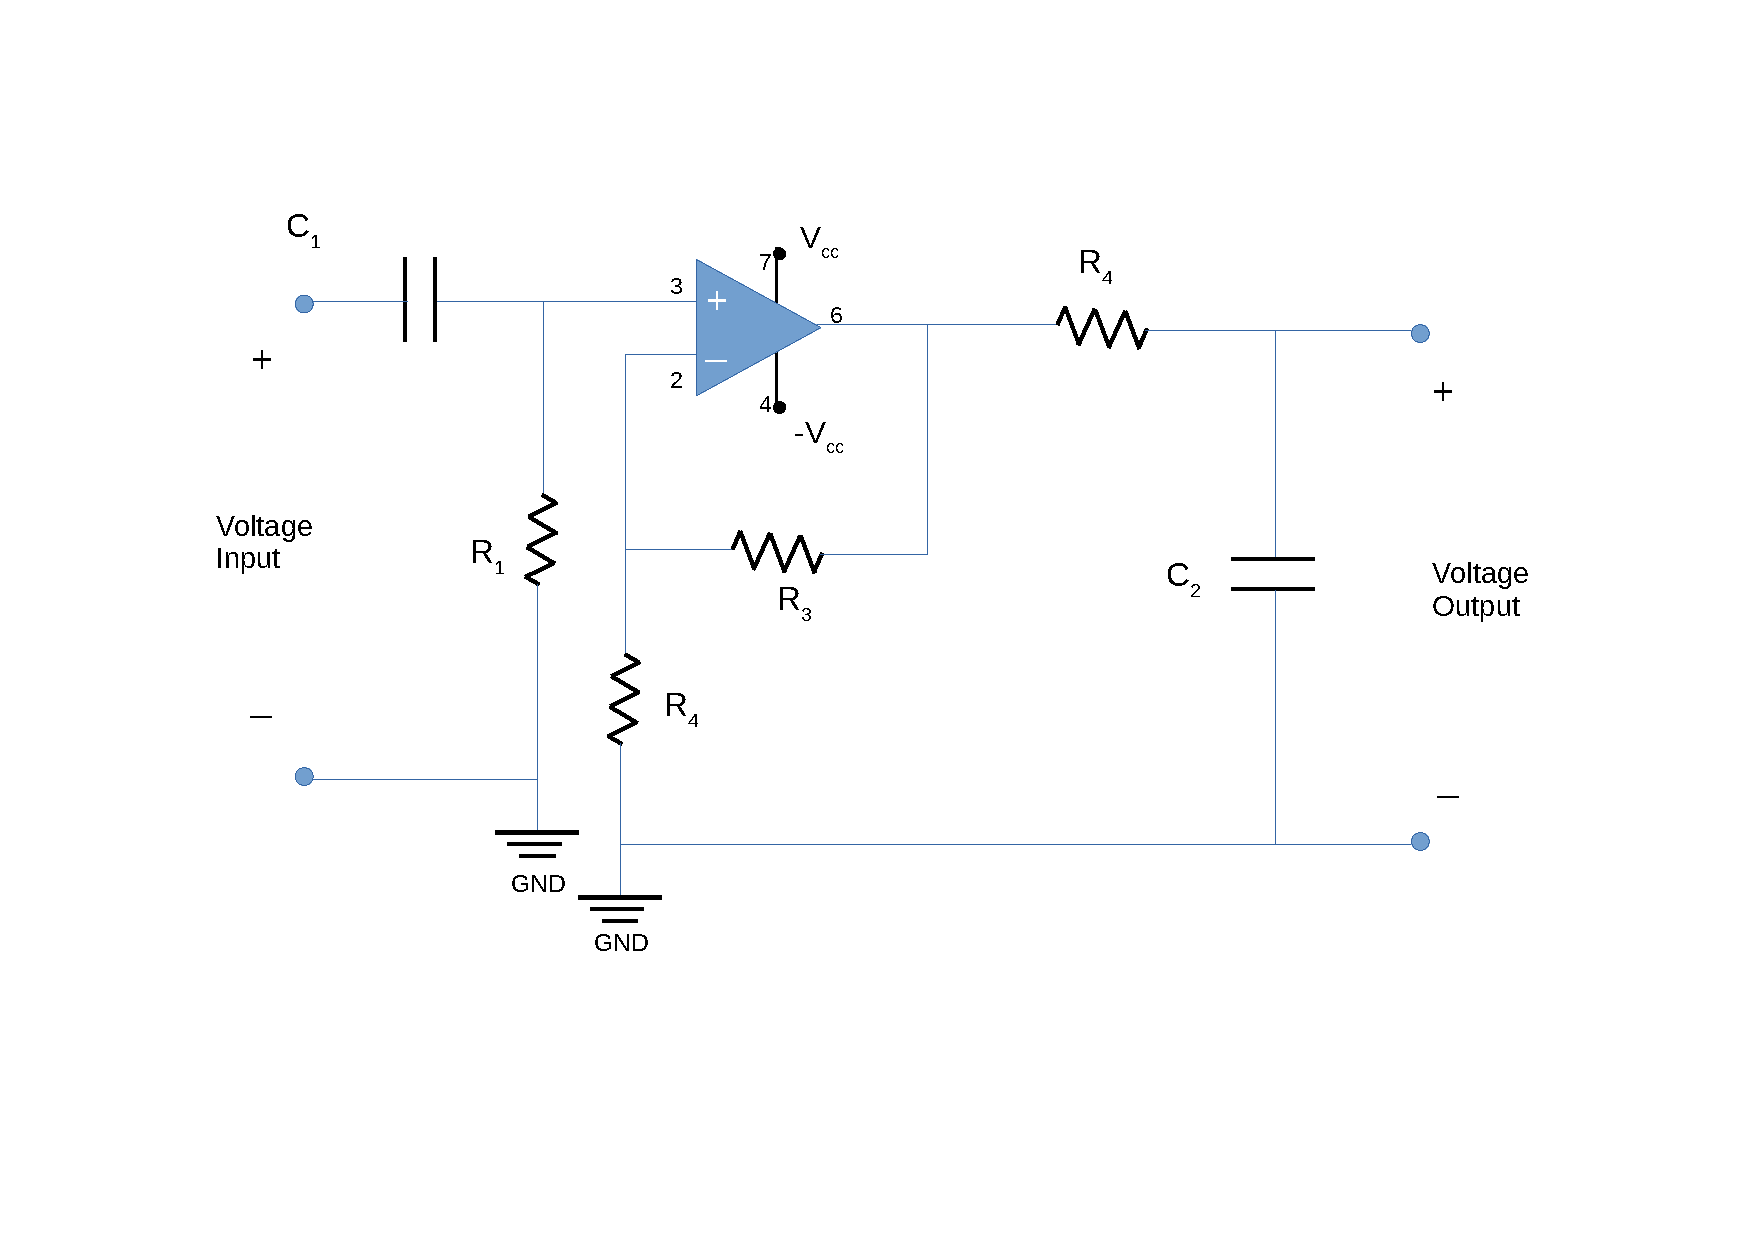
\includegraphics[width=0.95\linewidth]{DesenhoT5.pdf}
\caption{Representation of the BandPass Filter implemented.}
\label{fig:DesenhoT5}
\end{figure}

In this section we will discuss the theoretical analysis of our circuit, represented in figure \ref{fig:DesenhoT5}. The value for the central frequency is 1000Hz and the gain at the central frequency is 40db throughout the calculations. The ideal op-amp model is used so that $Z_input$ is infinite and $Z_ouput$ is null.

The values for the resistors and capacitors used are in table \ref{tab:values}. The first part of the circuit composed of $R_1$ and $C_1$ form the high-pass filter. It passes all frequencies above the value from equation ~\ref{eq:f1}. The signal is then amplified by the op amp by a gain proportional to resistors R3 and R4 according to the following equation. This means the gain is equal to ??.
\begin{table}[h]
    \centering
    \begin{tabular}{|l|c|}
    \hline
    {\bf Symbol} & {\bf Value} \\ \hline
    $R_{1}$ & $\Omega$ \\ \hline
    $R_{2}$ & $\Omega$ \\ \hline
    $R_{3}$ & $\Omega$  \\ \hline
    $R_{4}$ & $\Omega$\\ \hline
    $C_{1}$ & $\Omega$\\ \hline
    $C_{2}$ & $\Omega$\\ \hline
    \end{tabular}
    \caption{Values for theoretical analysis}
    \label{tab:values}
\end{table}

\begin{equation}
  Gain = 1+ \frac{R_3}{R_4},
  \label{eq:gain}
\end{equation}
\begin{equation}
  {f} = \frac{1}{2\pi*R_2*C_2},
  \label{eq:f1}
\end{equation}

The signal then passes through the low-pass filter, which is the second part of the circuit. The low-pass filter is composed of the resistor $R_2$ and capacitor $C_2$. It passes all frequencies below the value from the following equation. This circuit gives an amplified noinverting signal so the input signal and output signal are in phase.
\begin{equation}
  {f} = \frac{1}{2\pi*R_2*C_2},
  \label{eq:f2}
\end{equation}



Here we have the table for the values of the gain, input and output impedances calculated at the central frequency and the corresponding equations. 


\begin{equation}
|Z_input| = |\infty // Z_{C_1} + R_1| = |Z_{C_1} + R1|
\label{eq:impendances1}
\end{equation}

\begin{equation}
|Z_output| = |Z_{C_2} // (0 // R2 + R3)| = |Z_{C_2} // R2|
\label{eq:impendances2}
\end{equation}

\begin{table}[h]
    \centering
    \begin{tabular}{|l|c|}
    \hline
    {\bf Symbol} & {\bf Value} \\ \hline
    $Gain$ & ?? \\ \hline
    $Z_{input}$ & ?? \\ \hline
    $Z_{output}$ & ??  \\ \hline

    \end{tabular}
    \caption{Values for the gain, input and output impedances}
    \label{tab:valuesimp}
\end{table}

Finally, we can obtain the plot for the frequency response $V_o$(f)/$V_i$(f) using the incremental circuit, solving the circuit for a frequency vector in log scale with 10 points per decade, from 10Hz to 100MHz.

%%\begin{figure}[!ht] \centering
%%\caption{Frequency response $V_o$(f)/$V_i$(f)}
%\squeezeup  
%\includegraphics[width=0.8\linewidth]{??}
%\label{fig:theoretical}
%\end{figure}


  





